\section{Adaptive Stochastic Optimization} \label{sec:problem-statment}
We start by introducing notation and defining the general class of adaptive optimization problems that we address in this paper. For sake of clarity, we will illustrate our notation using the sensor placement application mentioned in \secref{sec:intro}. We give examples of other applications in~\secref{sec:stochastic-maximization},~\secref{sec:stochastic-set-cover},~\secref{sec:viral-marketing},
and~\secref{sec:active-learning}. 

\subsection{Items and Realizations} Let $\groundset$ be a finite set
of items (e.g., sensor locations).  Each item $\elem\in\groundset$ is
in a particular (initially unknown) state from a set $\outcomes$ of
possible states 
(describing whether a sensor
placed at location $\elem$ would malfunction or not). 
We represent the item states using a
function $\rlz:\groundset\rightarrow\outcomes$, called a 
\emph{realization} (of the states of all items in the ground set).
Thus, we say that $\rlz(\elem)$ is the state of $\elem$ under
realization $\rlz$.
We use $\rvrlz$ to denote a random realization. 
We take a Bayesian approach and assume that there is a known prior
probability distribution $\rlzprior := \Pr{\rvrlz = \rlz}$ over realizations (e.g., modeling
that sensors fail independently with failure probability), so that 
we can compute posterior distributions\footnote{In some situations, we
may not have exact knowledge of the prior $\rlzprior$.  Obtaining
algorithms that are robust to incorrect priors remains an interesting
source of open problems.  We briefly discuss some robustness
guarantees of our algorithm in~\secref{sec:the-greedy-policy} on page~\pageref{sec:robustness}.}.
%
We will consider problems where we sequentially pick an item
$\elem\in\groundset$, get to see its state $\rvrlz(\elem)$, pick the
next item, get to see its state, and so on (e.g., place a sensor, see whether it fails, and so on).  After each pick, our
observations so far can be represented as a \emph{partial realization}
$\prlz$, a function from some
subset of $\groundset$ (i.e., the set of items that we already picked)
to their states (e.g., $\prlz$ encodes where we placed sensors and which of them failed).  
For notational convenience, we sometimes represent  $\prlz$ as a relation, so that $\prlz \subseteq \groundset \times \outcomes$ equals 
$\set{(\elem, \outcome) : \prlz(\elem) = \outcome }$.
We use the notation $\dom(\prlz)=\set{\elem: \exists \outcome. (\elem,\outcome)\in\prlz}$ to refer to the domain of $\prlz$ (i.e., the set of items observed in $\prlz$).
A partial realization $\prlz$ is \emph{consistent}
with a realization $\rlz$ if they are equal everywhere in the domain
of $\prlz$.  
In this case we write $\rlz\sim\prlz$.  
If $\prlz$ and $\prlz'$ are both consistent with some $\rlz$, and 
$\dom(\prlz) \subseteq \dom(\prlz')$, we say $\prlz$ is a \emph{subrealization}
of $\prlz'$.  Equivalently, $\prlz$ is a subrealization
of $\prlz'$ if and only if, when viewed as relations, $\prlz \subseteq \prlz'$. 


Partial realizations are similar to the notion of ``belief states'' in
Partially Observable Markov Decision Problems (POMDPs), as they encode
the effect of all actions taken (items selected) and observations made, and determine our
posterior belief about the state of the world (i.e., the state of all
items $e$ not yet selected, $\rlzmass{\rlz \mid \prlz } := \Pr{\rvrlz =
  \rlz \mid \rvrlz \sim \prlz}$).

\subsection{Policies} We encode our adaptive strategy for picking items as a \emph{policy}
$\policy$, which is a function from a set of partial realizations to
$\groundset$, specifying which item to pick next under a particular
set of observations (e.g., $\policy$ chooses the next sensor location
given where we have placed sensors so far, and whether they failed or
not). 
We also allow randomized policies that are functions 
from a set of partial realizations to distributions on $\groundset$,
though our emphasis will primarily be on deterministic policies.
If $\prlz$ is not in the domain of $\policy$, the policy
terminates (stops picking items) upon observation of $\prlz$.
We use $\dom(\policy)$ to denote the domain of $\policy$.
Technically, we require that $\dom(\policy)$ be closed under
subrealizations.  That is, if $\prlz' \in \dom(\policy)$ and $\prlz$
is a subrealization of $\prlz'$ then $\prlz \in \dom(\policy)$.  
We use the notation $\played{\policy}{\rlz}$ to refer to the set of items selected by $\policy$ under realization $\rlz$.  Each deterministic policy $\policy$ can be associated with a decision
tree $T^{\policy}$ in a natural way (see \figref{fig:policyastree} for
an illustration).  
Here, we adopt a policy-centric view that admits concise
notation, though we find the decision tree view to be valuable conceptually.

Since partial realizations are similar to POMDP belief states, our definition of policies is similar to the notion of policies in POMDPs, which are usually defined as functions from belief states to actions. We will further discuss the relationship between the stochastic optimization problems considered in this paper and POMDPs in Section~\ref{sec:related-work}.

  \begin{figure} 
 \centering 
 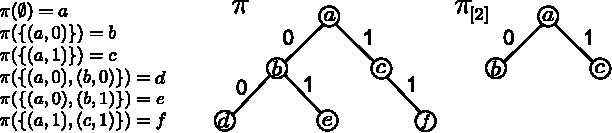
\includegraphics[width=0.85\textwidth]{figs/policyAsTree}
 \caption{Illustration of a policy $\policy$, its corresponding
   decision tree representation, and the decision tree representation
   of $\prune{\policy}{2}$, the level $2$ truncation of $\policy$
   (as defined in \secref{ssec:max-cover-objective}).}
%
\label{fig:policyastree}
 \end{figure}



\subsection{Adaptive Stochastic Maximization, Coverage, and Min-Sum Coverage} We wish to maximize, subject to some constraints, a utility function $f :2^{\groundset} \times \outcomes^\groundset \to \NonNegativeReals$ that depends on which items we pick and which state each item is in (e.g., modeling the total area covered by the working sensors).   
Based on this notation, the expected utility of a policy $\policy$ is
$\avgf(\policy) := \expctoverrlz{\rvrlz}{f(\played{\policy}{\rvrlz},
  \rvrlz)}$ where the expectation is taken with respect to $\rlzprior$.
The goal of the \emph{Adaptive Stochastic Maximization} problem is to 
find a policy $\policy^{*}$ such that 
\begin{equation}\policy^{*}\in\argmax_{\policy} \avgf(\policy) \text{
    subject to } |\played{\policy}{\rlz}|\leq \budget\text{ for all }\rlz, 
\label{eq:stochmax}\end{equation} where $\budget$ is a budget on how many items can be picked (e.g., we would like to adaptively choose $k$ sensor locations such that the working sensors provide as much information as possible in expectation).

\ifthenelse{\boolean{istechrpt}}{
Alternatively, we can specify a quota $\quota$ of utility that we
would like to obtain, and try to find the cheapest policy achieving
that quota (e.g., we would like to achieve a certain amount of information, as cheaply as possible in expectation). Formally, we define the average cost $\acst{\policy}$ of a
policy as the expected number of items it picks, so that
$\acst{\policy}:=\expctoverrlz{\rvrlz}{|\played{\policy}{\rvrlz}|}$. Our goal is then to find
\begin{equation}
\policy^{*}\in\argmin_{\policy} \acst{\policy}\text{ such that } f(\played{\policy}{\rlz},\rlz)\geq \quota\text{ for all }\rlz,\label{eq:stochcover}
\end{equation}
i.e., the policy $\policy^{*}$ that minimizes the expected number of
items picked such that under all possible realizations, at least
utility $Q$ is achieved. We call Problem~\ref{eq:stochcover} the
\emph{Adaptive Stochastic Minimum Cost Cover} problem.  We will also
consider the problem where we want to minimize the worst-case cost
$\wcst{\policy}:=\max_{\rlz}{|\played{\policy}{\rlz}|}$.  This
worst-case cost $\wcst{\policy}$ is the cost
incurred under adversarially chosen realizations, or  equivalently the
depth of the deepest leaf in $T^{\policy}$, the decision tree
associated with $\policy$.   



Yet another important variant is to minimize the average time required
by a policy to obtain its utility.  Formally, let $\util{\policy}{t}$ be
the expected utility obtained by $\policy$ after $t$
steps\footnote{For a more formal definition of $\util{\policy}{t}$,
  see \secref{sec:proofs-min-sum-cover} on page~\pageref{sec:proofs-min-sum-cover}.},
let $\quota = \expctoverrlz{\rlz}{f(\groundset, \rvrlz)}$ be the maximum
possible expected utility, 
and define the \emph{min-sum cost} $\costminsum{\policy}$ of a policy as 
$\costminsum{\policy} := \sum_{t = 0}^{\infty} \paren{
\quota -  \util{\policy}{t}}$.  We then define the  \emph{Adaptive
Stochastic Min-Sum Cover} problem as the search for
\begin{equation}
\policy^{*} \in \argmin_{\policy} \costminsum{\policy}. \label{eq:minsumcover}
\end{equation}



Unfortunately, as we will show in \secref{sec:hardness}, even for
linear functions $f$, i.e., those where $f(A,\rlz)=\sum_{\elem\in
  A}w_{\elem,\rlz}$ is simply the sum of weights (depending on the
realization $\rlz$), Problems~(\ref{eq:stochmax}),  (\ref{eq:stochcover}),
and (\ref{eq:minsumcover})  
are hard to approximate 
under reasonable complexity theoretic assumptions. 
Despite the hardness of the general problems, 
in the following sections we will identify conditions that are sufficient to 
allow us to approximately solve them.
}{
%
Unfortunately, as we will show in \secref{sec:hardness}, even for
linear functions $f$, i.e., those where $f(A,\rlz)=\sum_{\elem\in
  A}w_{\elem,\rlz}$ is simply the sum of weights (depending on the
realization $\Phi$), Problems~(\ref{eq:stochmax})
is hard to approximate under reasonable complexity theoretic
assumptions.
Despite the hardness of the general problem, 
in the following sections we will identify conditions that are sufficient to 
allow us to approximately solve it.
}



%
\subsection{Incorporating Item Costs}  
Instead of quantifying the cost of a set $\played{\policy}{\rlz}$ by
the number of elements $|\played{\policy}{\rlz}|$, we can also
consider the case where each item $\elem\in\groundset$ has a 
cost $c(\elem)$, and the cost of a set
$S\subseteq\groundset$ is $c(S)=\sum_{\elem\in S}c(\elem)$. We can
then consider variants of
Problems~\eqref{eq:stochmax},~\eqref{eq:stochcover},
and~\eqref{eq:minsumcover} with the $|\played{\policy}{\rlz}|$
replaced by 
$c(\played{\policy}{\rlz})$. For clarity of presentation, we will focus on the unit cost case, i.e., $c(\elem)=1$ for all $e$, 
and explain how our results generalize to the non-uniform case in \appendixA.

 


%
%
%
%
%
